\documentclass[usenames,dvipsnames]{beamer}
\usepackage[utf8]{inputenc}
\usepackage[T1]{fontenc}
\usepackage[french]{babel}
\usepackage{xcolor}
\usepackage{pifont}
\usepackage{float}
\usepackage{amsmath}
\usetheme{Boadilla} %Boadilla | Bergen | Madrid | Antibes | Hannover | Singapore | Warsaw | Montpellier

\newcommand{\cmark}{\ding{51}}
\newcommand{\xmark}{\ding{55}}
\newcommand*\mean[1]{\overline{#1}}

\setcounter{tocdepth}{1}
%----------------------------------------------------------------------------------------
%   TITLE INFORMATION
%----------------------------------------------------------------------------------------
\title{Analyse de sentiments}
\subtitle{HMIN232M -- Méthodes de la science des données}
\author{B. Rima \and E. Youssef \and T. Shaqura}
\institute[UM]{M1 Informatique AIGLE}
\date{25 avril 2019}

\begin{document}
%----------------------------------------------------------------------------------------
%   TITLE FRAME
%----------------------------------------------------------------------------------------
\begin{frame}
\titlepage
\end{frame}
%----------------------------------------------------------------------------------------
%   OUTLINE
%----------------------------------------------------------------------------------------
\begin{frame}{Sommaire}
\tableofcontents
\end{frame}
%----------------------------------------------------------------------------------------
%   INTRODUCTION
%----------------------------------------------------------------------------------------
\section{Pré-traitements}
\subsection{Préparation à la tokenization}
\begin{frame}{Préparation à la tokenization}{Pré-traitements}
\begin{figure}[!ht]
  \centering
  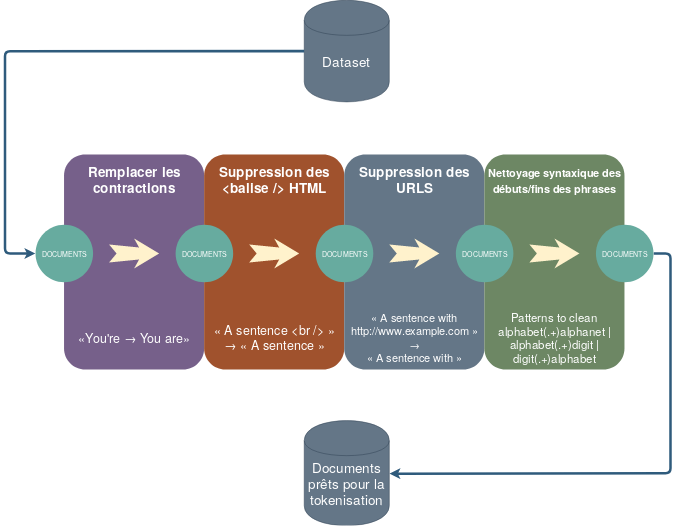
\includegraphics[scale=0.35]{images/preparation_tokenization.png}
\end{figure}
\end{frame}

\subsection{Tokenisation et normalisation}
\begin{frame}{Tokenisation et normalisation}{Pré-traitements}
\begin{figure}[!ht]
  \centering
  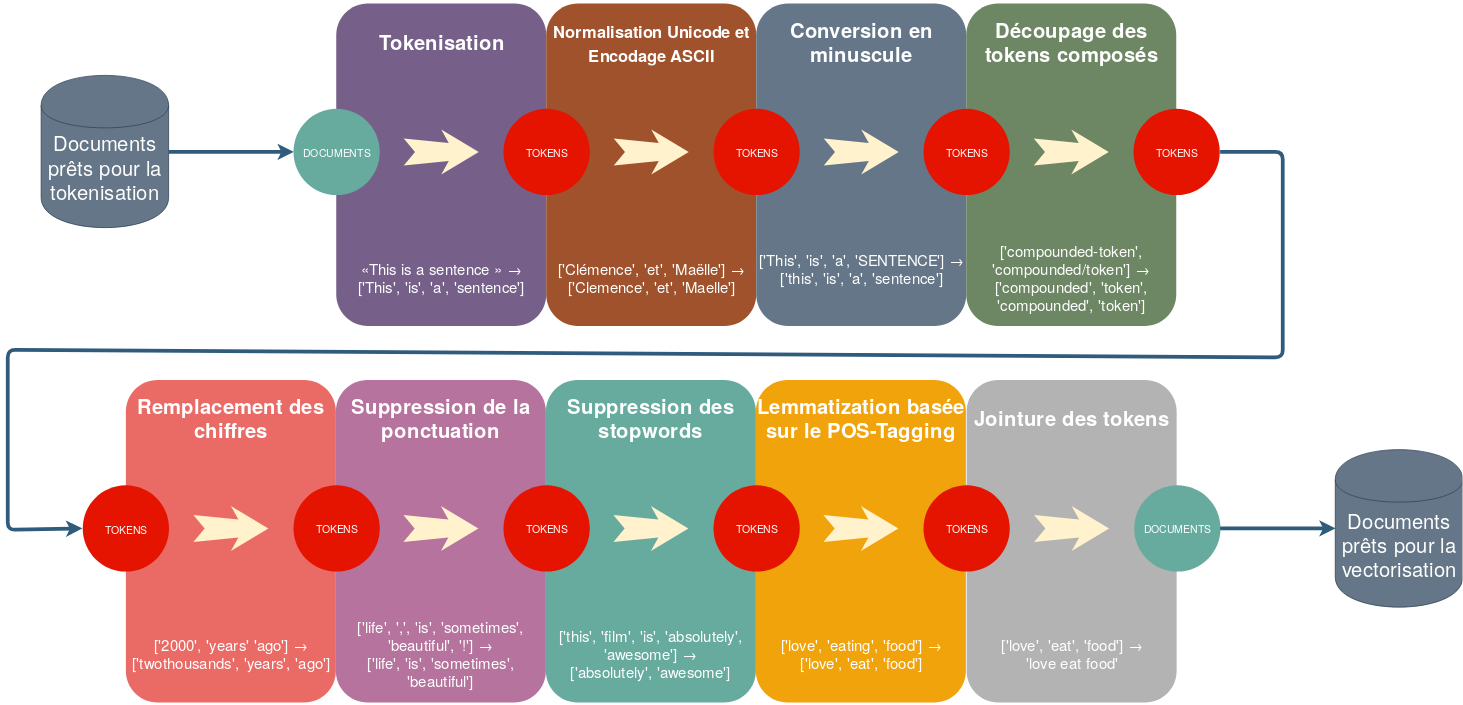
\includegraphics[scale=0.2]{images/tokenization_normalization.png}
\end{figure}
\end{frame}

\section{Visualisation des données}
\subsection{WordCloud}
\begin{frame}{WordCloud}{Visualisation des données}
\begin{columns}
\column{0.5\textwidth}
\begin{figure}
    \centering
    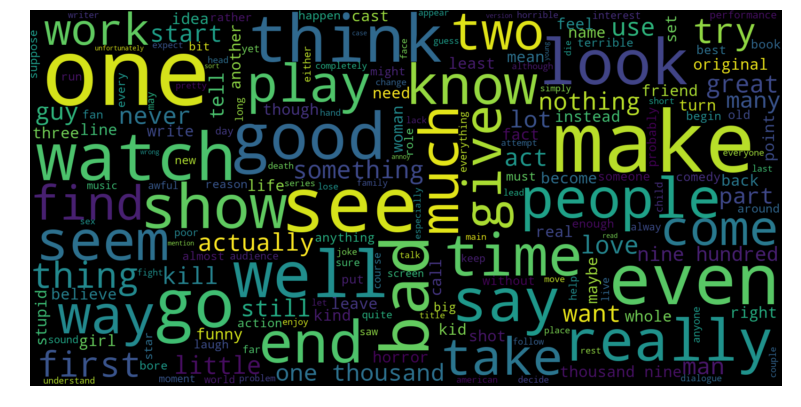
\includegraphics[width=1.0\textwidth]{images/negative_opinions_frequent_words.png}
    \caption{Les mots les plus fréquents dans les avis négatifs}
\end{figure}
\column{0.5\textwidth}
On peut s'attendre à...
\begin{itemize}
    \item Beaucoup d'ironies
    \item Phrases à polarités différentes dans les avis
\end{itemize}
\end{columns}
\end{frame}

\section{Vectorisation et sélection des features}
\begin{frame}{Vectorisation et sélection des features}
\begin{figure}
    \centering
    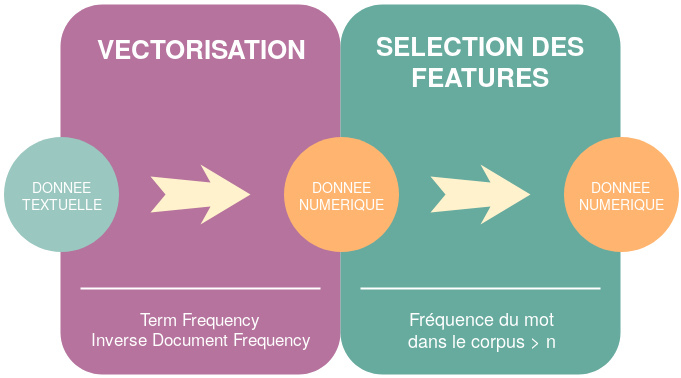
\includegraphics[scale=0.3]{images/features.png}
    \caption{Traitement des features}
    \label{fig:features}
\end{figure}
\end{frame}

\section{Cross-validation}
\subsection{Principe}
\begin{frame}{Principe}{Cross-validation}
\begin{figure}[!ht]
  \centering
  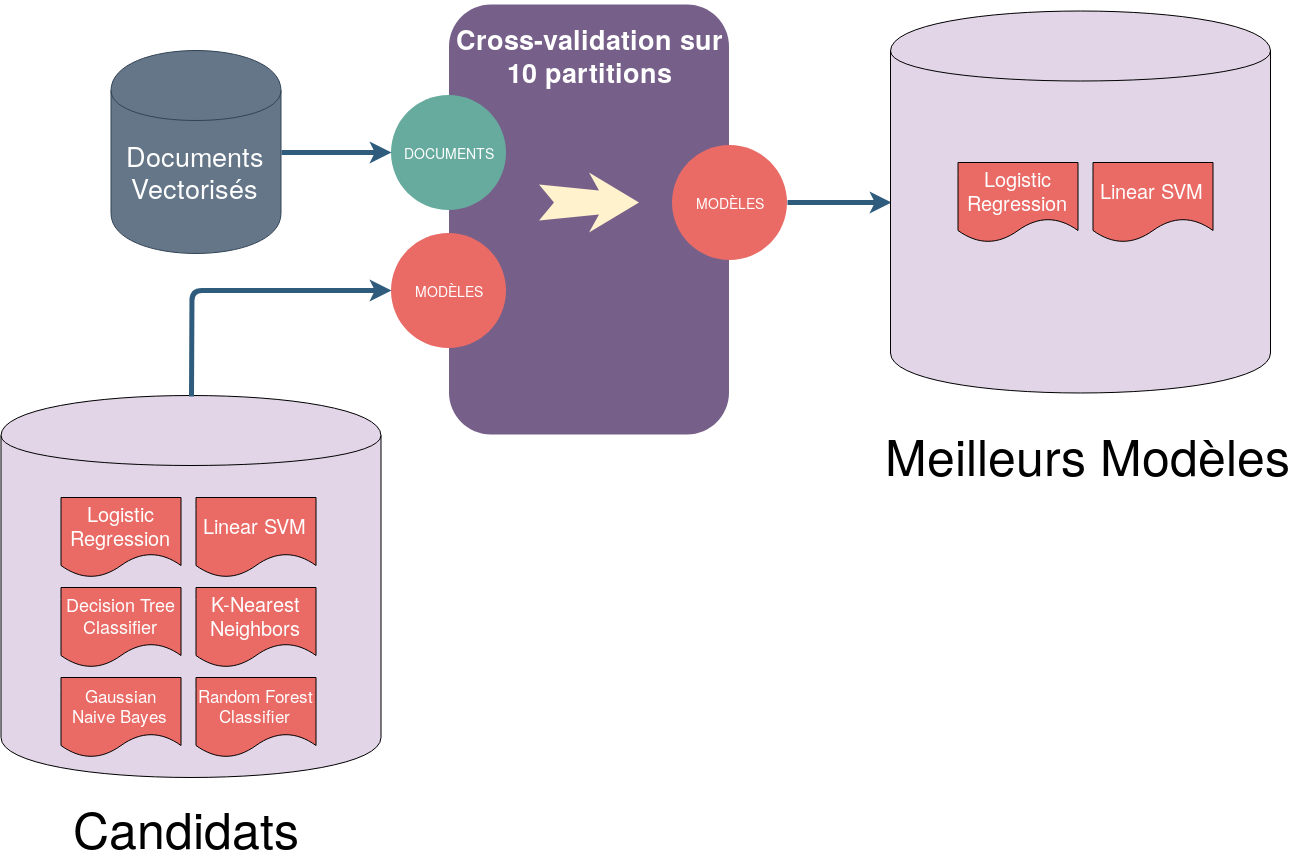
\includegraphics[scale=0.2]{images/cross_validation.png}
\end{figure}
\end{frame}

\subsection{Résultats de la cross-validation}
\begin{frame}{Résultats de la cross-validation}{Cross-validation}
\begin{table}
  \centering
  \begin{tabular}{|p{5cm}|c|c|}
    \hline
    \textbf{Modèle} & $\mean{score}$ & $\sigma$\\
    \hline
    \hline
    LinearSVC & 92\% & 1\%\\
    \hline
    SGDClassifier & 92\% & 1\%\\
    \hline
    LogisticRegression & 91\% & 0.8\%\\
    \hline
    GaussianNB & 84\% & 1\%\\
    \hline
    RandomForestClassifier & 81\% & 1\%\\
    \hline
    KNeighborsClassifier & 79\% & 1\%\\
    \hline
    DecisionTreeClassifier & 75\% & 0.8\%\\
    \hline
  \end{tabular}
\end{table}
\end{frame}

\section{Calibrage des hyperparamètres}
\subsection{Principe}
\begin{frame}{Principe}{Calibrage des hyperparamètres}
\end{frame}

\subsection{Résultats du calibrage}
\begin{frame}{Résultats du calibrage}{Calibrage des hyperparamètres}
\begin{tabular}{|p{5cm}|c|c|}
  \hline
  \textbf{Modèle} & $\mean{score}$ & \textbf{Meilleurs calibrages}\\
  \hline
  \hline
  LogisticRegression & 90\% & C = 11.288 ; penalty = $L_2$\\
  \hline
  LinearSVC & 90\% & C = 1\\
  \hline
\end{tabular}
\end{frame}

\section{Création des pipelines}
\subsection{Pipeline pour Logistic Regression}
\begin{frame}{Pipeline pour Logistic Regression}{Création des pipelines}
\begin{figure}[!ht]
  \centering
  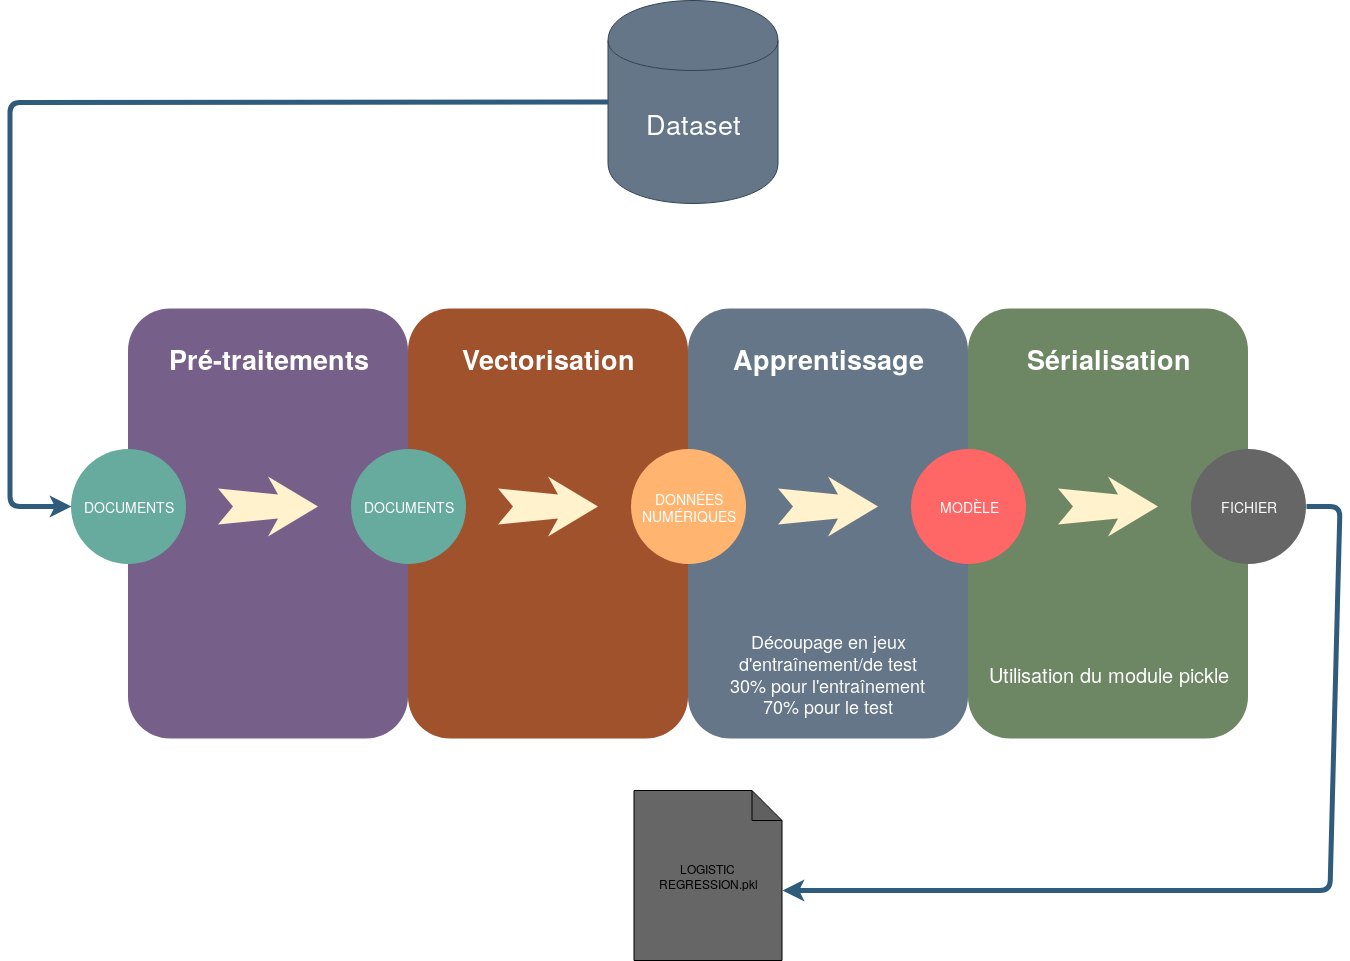
\includegraphics[scale=0.18]{images/pipeline_logistic_regression.png}
\end{figure}
\end{frame}

\subsection{Résultats pour le dataset du challenge}
\begin{frame}{Résultats pour le dataset du challenge}{Création des pipelines}
\begin{figure}[!ht]
  \centering
  \textbf{Accuracy} : 89\% \\
  \textbf{Temps pour effectuer la prédiction} $\approx41$ secondes.
  $$
  \begin{pmatrix}
  1770 & 230 \\
  190 & 1810
  \end{pmatrix}
  $$
\end{figure}

\begin{table}
  \centering
  \begin{tabular}{|c|c|c|c|c|}
    \hline
    \textbf{Value} & \textbf{Precision} & \textbf{Recall} & \textbf{F1-score} & \textbf{Support}\\
    \hline
    \hline
    -1 & 90\% & 89\% & 89\% & 2000\\
    \hline
    1 & 89\% & 91\% & 90\% & 2000\\
    \hline
    Micro avg & 90\% & 90\% & 90\% & 4000\\
    \hline
    Macro avg & 90\% & 90\% & 89\% & 4000\\
    \hline
    Weighted avg & 90\% & 90\% & 89\% & 4000\\
    \hline
  \end{tabular}
\end{table}
\end{frame}

\subsection{Résultats pour le dataset IMDB}
\begin{frame}{Résultats pour le dataset IMDB}{Création des pipelines}
\begin{figure}[!ht]
  \centering
  \textbf{Accuracy} : 85\% \\
  \textbf{Temps pour effectuer la prédiction} $\approx106$ secondes.
  $$
  \begin{pmatrix}
  4107 & 893 \\
  602 & 4398
  \end{pmatrix}
  $$
\end{figure}

\begin{table}
  \centering
  \begin{tabular}{|c|c|c|c|c|}
    \hline
    \textbf{Value} & \textbf{Precision} & \textbf{Recall} & \textbf{F1-score} & \textbf{Support}\\
    \hline
    \hline
    -1 & 87\% & 82\% & 85\% & 5000\\
    \hline
    1 & 83\% & 88\% & 85\% & 5000\\
    \hline
    Micro avg & 85\% & 85\% & 85\% & 10000\\
    \hline
    Macro avg & 85\% & 85\% & 85\% & 10000\\
    \hline
    Weighted avg & 85\% & 85\% & 85\% & 10000\\
    \hline
  \end{tabular}
\end{table}
\end{frame}

\subsection{Pipeline pour Gaussian Naive Bayes}
\begin{frame}{Pipeline pour Gaussian Naive Bayes}{Création des pipelines}
\begin{figure}[!ht]
  \centering
  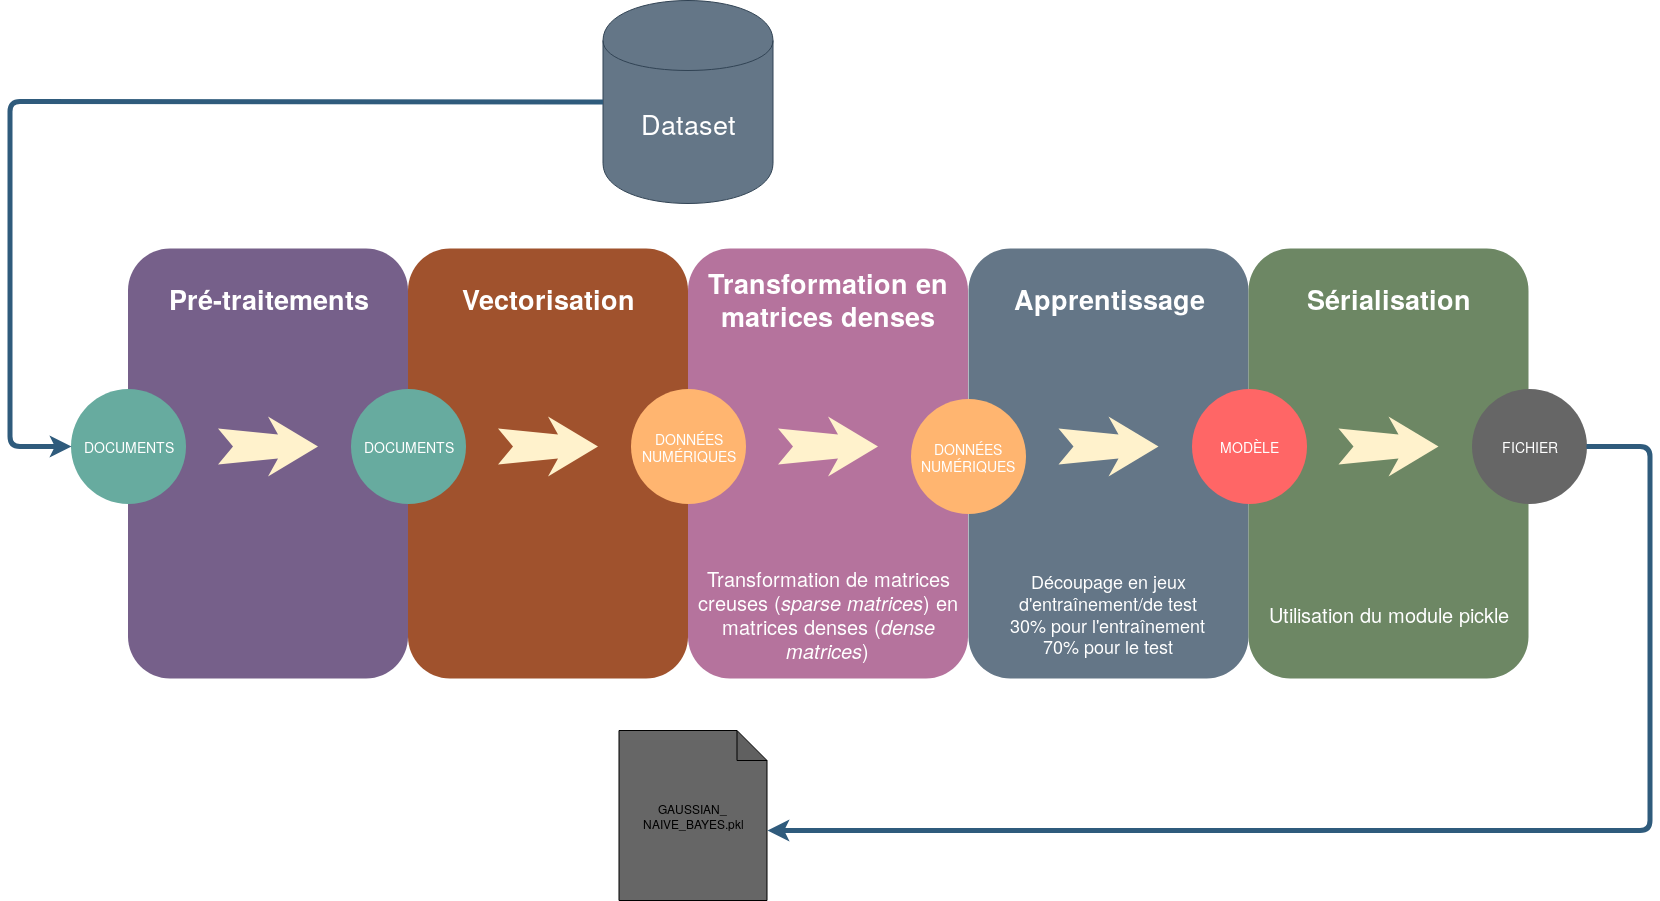
\includegraphics[scale=0.18]{images/pipeline_gaussian_naive_bayes.png}
\end{figure}
\end{frame}

\subsection{Résultats pour le dataset du challenge}
\begin{frame}{Résultats pour le dataset du challenge}{Création des pipelines}
\begin{figure}[!ht]
  \centering
  \textbf{Accuracy} : 84\% \\
  \textbf{Temps pour effectuer la prédiction} $\approx42$ secondes.
  $$
  \begin{pmatrix}
  1666 & 334 \\
  290 & 1710
  \end{pmatrix}
  $$
\end{figure}

\begin{table}
  \centering
  \begin{tabular}{|c|c|c|c|c|}
    \hline
    \textbf{Value} & \textbf{Precision} & \textbf{Recall} & \textbf{F1-score} & \textbf{Support}\\
    \hline
    \hline
    -1 & 85\% & 83\% & 84\% & 2000\\
    \hline
    1 & 84\% & 85\% & 85\% & 2000\\
    \hline
    Micro avg & 84\% & 84\% & 84\% & 4000\\
    \hline
    Macro avg & 84\% & 84\% & 84\% & 4000\\
    \hline
    Weighted avg & 84\% & 84\% & 84\% & 4000\\
    \hline
  \end{tabular}
\end{table}
\end{frame}

\subsection{Résultats pour le dataset IMDB}
\begin{frame}{Résultats pour le dataset IMDB}{Création des pipelines}
\begin{figure}[!ht]
  \centering
  \textbf{Accuracy} : 77\% \\
  \textbf{Temps pour effectuer la prédiction} $\approx106$ secondes.
  $$
  \begin{pmatrix}
  3634 & 1366 \\
  914 & 4086
  \end{pmatrix}
  $$
\end{figure}

\begin{table}
  \centering
  \begin{tabular}{|c|c|c|c|c|}
    \hline
    \textbf{Value} & \textbf{Precision} & \textbf{Recall} & \textbf{F1-score} & \textbf{Support}\\
    \hline
    \hline
    -1 & 80\% & 73\% & 76\% & 5000\\
    \hline
    1 & 75\% & 82\% & 78\% & 5000\\
    \hline
    Micro avg & 77\% & 77\% & 77\% & 10000\\
    \hline
    Macro avg & 77\% & 77\% & 77\% & 10000\\
    \hline
    Weighted avg & 77\% & 77\% & 77\% & 10000\\
    \hline
  \end{tabular}
\end{table}
\end{frame}

\section{Conclusion}
\subsection{Schéma globale de nos traitements}
\begin{frame}{Schéma globale de nos traitements}{Conclusion}
\begin{figure}
    \centering
    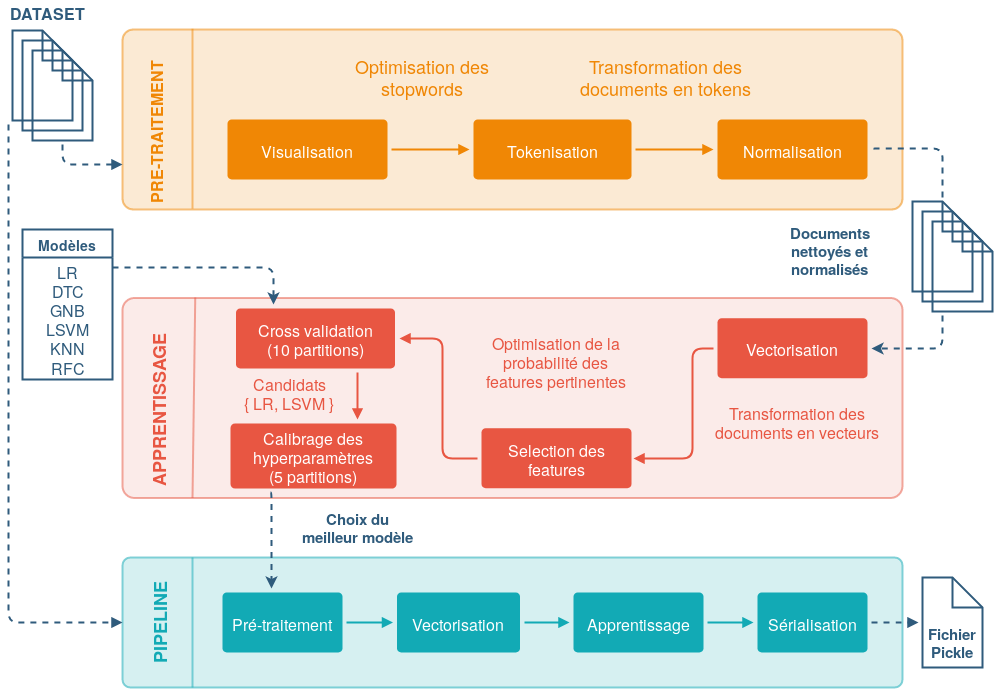
\includegraphics[scale=0.25]{images/conclusion.png}
\end{figure}
\end{frame}

\end{document}
